\documentclass[a4paper]{article}

\usepackage{array}
\usepackage{ctexcap}
\usepackage{ctex}
\usepackage{geometry}
\usepackage{graphicx}
\usepackage{amsmath,amssymb,lastpage,ulem,booktabs}
\usepackage{array,tabularx}
\usepackage{siunitx}
\usepackage{floatrow,calc}
\newcolumntype{C}{>{\hfil}X<{\hfil}}
\geometry{
    top=25mm, 
    left=25mm, 
    right=25mm, 
    bottom=25mm,
    headsep=10mm,
    footnotesep=7mm
}
\title{{\bfseries 电路理论基础实验} \\ \zihao{4}\songti 仪器入门及电位、电压的测量}
\author{材料科学与工程学院\\ 杨越\quad 22301071}
\date{}
\pagestyle{plain}

\begin{document}
\begin{center}
    {\mbox{}\\[7em]\zihao{2}\bfseries\songti%
    电路基础实验实验报告}\\[34mm]
    {\zihao{-3}\bfseries\songti
    实验名称:\uline{\hfill\mbox{仪器入门及电位、电压的测量}\hfill} \\[2.9mm]
    学\quad 号:\uline{\makebox[25mm]{22301071}}\hfill
    姓\quad 名:\uline{\makebox[25mm]{杨\quad 越}}\hfill
    班\quad 级:\uline{\makebox[25mm]{22级高分子}} \\[2.9mm]
    合作者:\uline{\makebox[25mm]{杨雨燃}}\hspace*{7.4mm}
    桌\quad 号:\uline{\makebox[25mm]{32}}\hfill\mbox{}\\[2.9mm]
    指导教师:\uline{\makebox[30mm]{张志鹏}}\hfill\mbox{} \\[2.9mm]
    实验日期:\uline{\makebox[30mm]{2024-04-30}}\hfill\mbox{} \\[58.7mm]

    }
\end{center}
\newpage

\section{实验目的}

\begin{enumerate}
    \item 了解万用表和直流稳压电源的基本功能并掌握其使用方法;
    \item 了解电路分析实验箱的基本构造并掌握其使用方法;
    \item 用实验证明电路中电位的相对性和电压的绝对性。
\end{enumerate}

\section{实验原理及电路图}
\begin{flushleft}
    \bfseries\zihao{-4}\songti 【实验原理】
\end{flushleft}
\begin{enumerate}
    \item 万用表\par 作用:测量电路中各种基本电参数(如:交流直流电压、电流、电阻阻值、电容等)\par 主要技术指标:测量精度(3\%,4\%,5\%,6\%等规格),5\% 第一位数只能显示0或1,称为半位。显示位数越多则分辨率越高,精度越高。\par 使用方法:\par
        \begin{enumerate}
            \item 选择功能
            \item 选择量程(手动或自动)
            \item 与元件连接测量对应参数
        \end{enumerate}
    \item 直流稳压电源\par 模式:分为CV(恒压输出),CC(恒流输出),UR(临界模式)三种输出模式,CV,CC各自对应其输出的电压值,电流值 \par 使用方法:\par
        \begin{enumerate}
            \item 选择通道
            \item 设置输出电压、电流
            \item 设置过压过流保护
            \item 打开输出
        \end{enumerate}
    \item 电路分析实验箱\par 用于进行电路分析实验。\par 具体分区:\par
        \begin{enumerate}
            \item 仪表区:提供直流电压表与直流毫安表
            \item 电源区:提供两路直流稳压电源,档位分别为0-10V与10-21V\par 使用简单、连接方便
            \item 实验电路区:组装实验电路
        \end{enumerate}
    \item 电位与电压的测量\par 电位差(电压)与参考点选择无关。\par 电位变化图:电路中的电位值为纵坐标,电路中各点位置为横坐标,将标出各点用直线相连。
\end{enumerate}
\begin{flushleft}
    \bfseries\zihao{-4}\songti 【实验电路图】
\end{flushleft}\par
实验一、二、三直接将万用表与待测电阻或二极管相连,此处省略其实验电路图。\par
实验四实验电路图如下图所示
\begin{center}
    \includegraphics*{1.url}\\
    \bfseries\zihao{5}\songti 图1:实验四电路图
\end{center}

\section{实验仪表}
实验中所用的仪表包括万用表、直流稳压电源与电路分析实验箱中的各种组件,其具体规格及使用方法已在实验原理中提及,此处不再赘述。

\section{实验内容及步骤}
\begin{enumerate}
    \item 测量实验箱中标称100Ω和1KΩ电阻阻值、标称0.1μ和2μ电容的电容值并记录,计算其绝对误差与相对误差。
    \item 万用表二极管档测量二极管导通情况,红表笔接二极管正极、黑表笔接二极管负极时导通,万用表显示其导通压降。测量实验箱中伏安特性单元二极管导通电压并记录。
    \item 设置直流稳压电源输出电压5V,输出电流50mA。将电源接入实验箱中伏安特性单元的200Ω电阻和51Ω电阻两端,观察稳压电源工作模式(CCorCV),记录。
    \item 参考实验原理部分中所示电路图连接电路。
    \begin{enumerate}
        \item 将稳压电源设置为5V,接入E1,另一稳压电源设为8V,接入E2。
        \item 分别以A,D为参考点测量B、C、D、E、F各点的电位值Φ及所有相邻两点电压值$ U_{AB} $、$ U_{BC} $、$ U_{CD} $、$ U_{DE} $、$ U_{EF} $、$ U_{FA} $,记录并完成表格。
        \item 
    \end{enumerate}
\end{enumerate}
\newpage

\section{实验结果}
    \songti\zihao{-4} 各个实验结果表如下所示\par
    \begin{table}[!ht]
        \caption{测量标称电容、电阻与二极管}\label{tab:exp4}
        \begin{tabularx}{\textwidth}{*{6}{C}} \toprule
            项目 & 电阻1 & 电阻2 & 电容1 & 电容2 & 二极管 \\ \midrule
            标称值 & 100$\Omega $ & 1k$\Omega $ & 0.1μF & 1μF & - \\ 测量值 & 98.654$\Omega $ & 990.20$\Omega $ & 0.1197μF & 1.036μF & 0.5555V \\ 绝对误差 & 1.346$\Omega $ & 9.8$\Omega $ & 0.0197μF & 0.036μF & - \\ 相对误差 & 1.346\% & 0.98\% & 19.7\% & 3.6\% & -  \\
            \bottomrule
        \end{tabularx}
    \end{table}
    \begin{table}[!ht]
        \caption{观察稳压电源的工作模式结果表}\label{tab:exp4}
        \begin{tabularx}{\textwidth}{*{4}{C}} \toprule
            负载电阻 & 工作模式 & 电压(V) & 电流(mA) \\ \midrule
            200$\Omega $ & CV & 5.012 & 26 \\  51$\Omega $ & CC & 2.511 & 50 \\ 
            \bottomrule
        \end{tabularx}
    \end{table}
    \begin{table}[!ht]
        \caption{实验四电位测量结果表}\label{tab:exp4}
        \begin{tabularx}{\textwidth}{*{7}{C}} \toprule
            电位(\unit{V}) & $\phi_A $ & $\phi_B $ & $\phi_C $ & $\phi_D $ &$\phi_E $ &$\phi_F $ \\ \midrule
            A & 0 & 2.4766 & -5.4849 & -3.0168 & -4.3111 & 0.7350 \\  D & 2.9988 & 5.5075 & -2.4503 & 0 & -1.20794 & 3.7956 \\
            \bottomrule
        \end{tabularx}
    \end{table}
    \begin{table}[!ht]
        \caption{实验四电位差(电压)测量结果表}\label{tab:exp4}
        \begin{tabularx}{\textwidth}{*{7}{C}} \toprule
            电位差(\unit{V}) & $U_{AB}$ & $U_{BC}$ & $U_{CD}$ & $U_{DE}$ & $U_{EF}$ & $U_{FA}$ \\ \midrule
            A & 2.4720 & -7.9599 & 2.4129 & -1.25615 & 5.0042 & -0.72187 \\  D & 2.4305 & -7.9609 & 2.37499 & -1.25329 & 5.0051 & -0.72304 \\
            \bottomrule
        \end{tabularx}
    \end{table}
    表格签名页附报告后。

\newpage

\section{实验结果与分析}
{\songti\zihao{-4}\bfseries 实验一、二误差的计算过程以及误差分析如下:}\par
\begin{enumerate}
    \item 绝对误差的计算:采用测量值与真实值作差取绝对值得到,即如下公式 $$ \epsilon = |x_i-x_r| $$ 
    \item 相对误差的计算:相对误差等于绝对误差除真实值,即如下公式 $$ \gamma = \frac{\epsilon}{x_r}×100\% = \frac{|x_i-x_r|}{x_r}×100\%  $$
    \item 以电阻1为例,假设其真实电阻值与标称值相等,用其标称值取代真实值进行计算,其测量值为98.654$\Omega $,则绝对误差为1.346$\Omega $,相对误差为 $ \frac{1.346}{100}×100\% = 1.346\% $
    \item 对实验结果的讨论以及影响实验结果的因素分析:\par 
        \begin{enumerate}
            \item 首先注意到测量电阻时其阻值相较于真实值略低,但相对误差较小,整体阻值变化不大。推测电阻随时间推移其阻值略有降低。
            \item 电容测量所得到的电容值相较于真实值偏高,不考虑测量本身带来的误差,则可能是待测电容两极板中相较原本掺有少量绝缘体导致其电容实际值增加。
            \item 二极管导通电压为0.5555V,反接后万用表显示OPEN,结果显示二极管导通性良好。
            \item 此外实验整体要考虑仪器自身测量带来的误差,人工读数引入的误差以及实验条件变化所带来的影响,如长时间通电会导致电阻温度升高,阻值与实际值相比偏高。
        \end{enumerate}
\end{enumerate}
\par
{\songti\zihao{-4}\bfseries 实验三的计算过程以及误差分析如下:}\par
\begin{enumerate}
    \item 当负载电阻为200$\Omega $时,根据欧姆定律$R=\frac{U}{I} $有,其实际测得的对应电阻阻值为192.77$\Omega $,相较于200$\Omega $偏低。同理可以得到后者对应阻值为50.22$\Omega $。
    \item 对于200$\Omega $的电阻,其工作模式为CV恒压模式,说明此时的输出电压达到了设定的电压。此时的电流小于恒压电源所设定的电流,说明若此时电源的输出电流按照设定电流进行输出,其阻值会大于其设定的输出电压值,故此时应当为CV恒压输出模式更为合理。
    \item 对于51$\Omega $的电阻,其工作模式为CC恒流模式,说明此时输出的电流与设定电流相同,同上若此时两端输出为设定电压,则其电流将会大于电源设定的输出电流值,故此时应当为CC恒流输出模式更为合理。
    \item 取两临界条件,即输出电压为5V,电流为0.050A,则求得此时对应临界模式UR的电阻阻值为100$\Omega $,与两电阻阻值对比,可得当待测电阻阻值高于UR对应电阻阻值,则其电源输出模式为CV;反之若小于UR对应电阻阻值,则其电源输出模式为CC。
    \item 同理,实验要考虑仪器自身带来的测量误差,人工读数导致的误差以及环境变化所导致的误差。
    \item 本实验电阻可以采用跟实验一同样的方法计算其绝对误差与相对误差如下,过程不再赘述。
    \begin{table}[!ht]
        \caption{实验三绝对误差、相对误差结果表}\label{tab:exp4}
        \begin{tabularx}{\textwidth}{*{3}{C}} \toprule
            负载电阻$\Omega $ & 200 & 51 \\ \midrule
            计算阻值/$\Omega $ & 192.77 & 50.22 \\  绝对误差/$\Omega $ & 7.23 & 0.78 \\  相对误差/\% & 3.62\% & 1.53\% \\ 
            \bottomrule
        \end{tabularx}
    \end{table}
\end{enumerate}
\par
{\songti\zihao{-4}\bfseries 实验四的结果分析以及误差分析如下:}\par
\begin{center}
    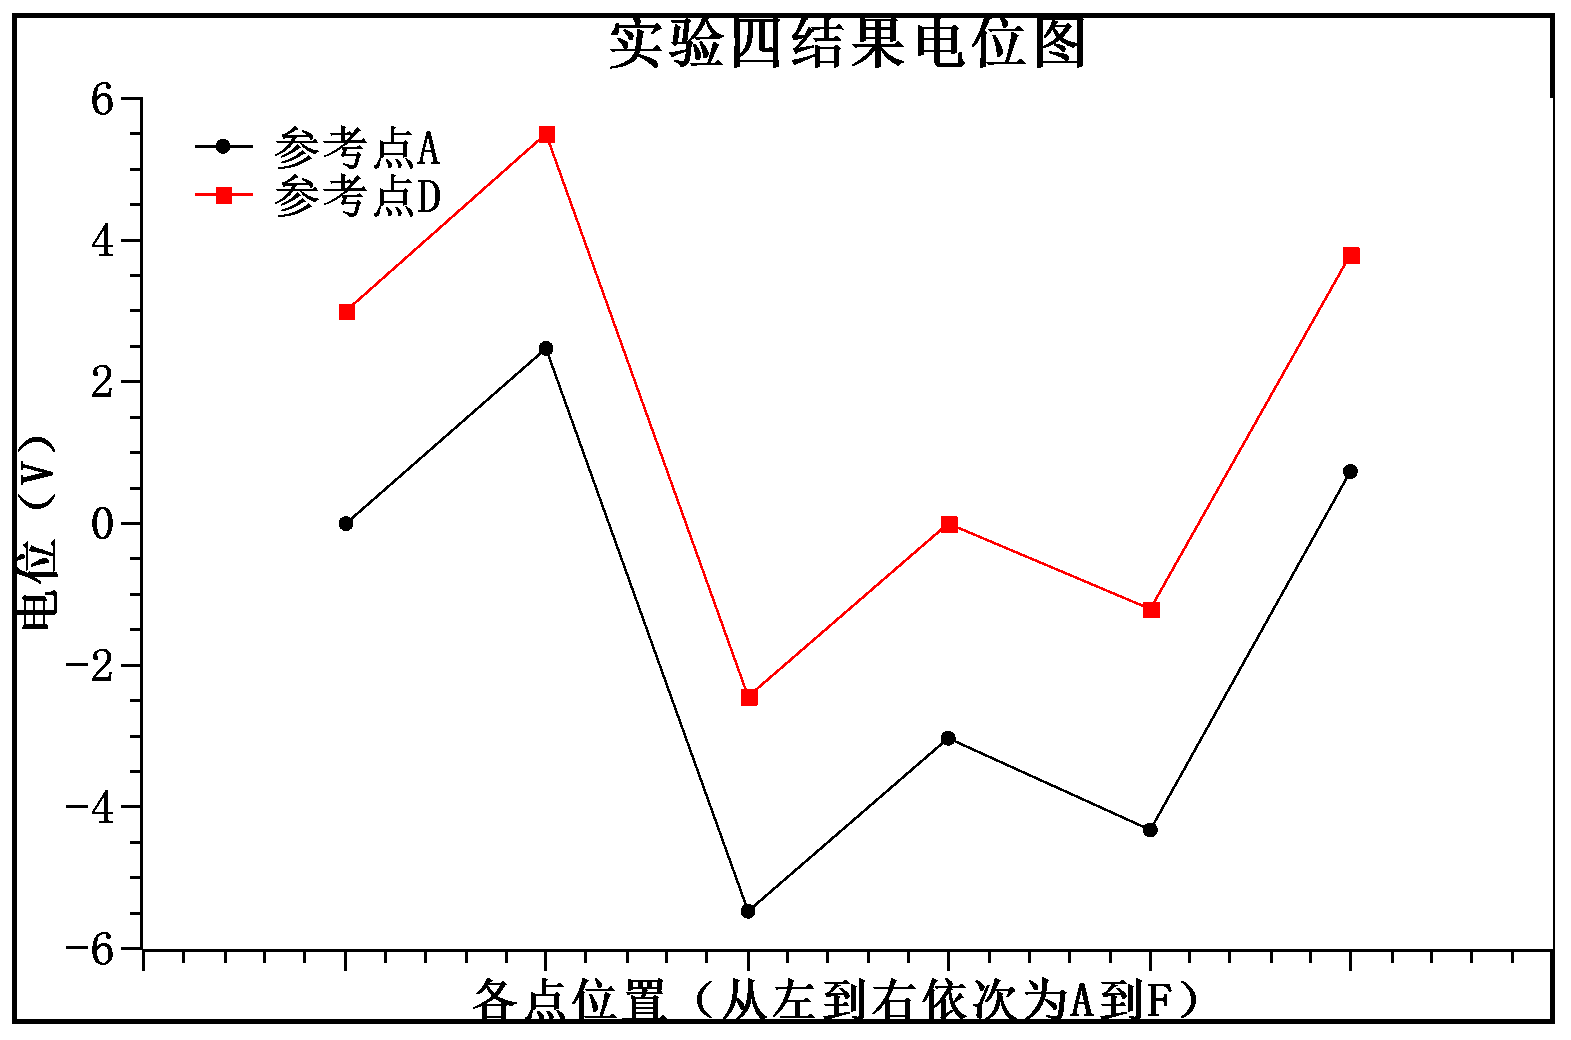
\includegraphics[width=\textwidth-40mm]{2.pdf}\\
    \bfseries\zihao{5}\songti 图2:实验四电位图
\end{center}
\begin{enumerate}
    \item 电位的相对性指:选取不同的参考点,其电位值会随之发生变化。根据实验结果得到电位图如上图所示,注意到两组数据对应的折线图可以视为上下发生平移得到,可以发现选取不同的参照点所得到的各点电位绝对值可能会发生改变,但彼此之间的相对走势,即相对值,维持不变,与电位的相对性的结论相印证。
    \item 电压的绝对性指:选取不同的参考点,两点之间的电位值的差值(即电压)不会随着参考点的变化而改变。对于本实验电路,选取任意两点电位值做差,发现其值大小几乎维持一致,不会随着参考点的选取发生变化。故电压的绝对性结论成立。
    \item 实验引入误差的环节同前,不再赘述。
\end{enumerate}

\section{思考题}
\subsection{总结电位相对性和电压绝对性的原理。}
电位相对性和电压绝对性二者已在前文分析过,此处进行总结。\par 电位相对性:对于电路中某一节点其电位值与参考的零势能点的选取相关联,而并不是一个恒定不变的量。\par 电压绝对性:对于电路中某两个节点的电位值之差(电势差,也即电压),其值与参考的零势能点的选取无关。对于电路中两点的电位作差,其所得的值理论上不随参考点的改变而改变,是恒定不变的。

\section{实验心得}
本次实验整体过程较为顺利,除了以前没有实际接触过类似的电路元件与仪器,导致找对应元件连接电路一步花费时间较长以外,其他部分没有明显问题。就个人而言,自己动手连接电路进行实验,得到对应的电路相关的结论的体验不错。\par
本次实验中的测量次数个人认为偏少,导致结果有较大概率引入偶然造成的误差。实际为了得到更加精确,更加具有可信度的实验结果,应当增加实验测量的次数,多次测量求取其平均值并进行误差分析。此外对于间接测量量可以进行误差传递等更加精确的误差处理得到其范围。\par
本次实验还可以进一步设计更多的电路图来对实验的目标结论,即电位相对性与电压绝对性进行验证,进一步增加结果的可信度。\par

\newpage
\begin{center}
    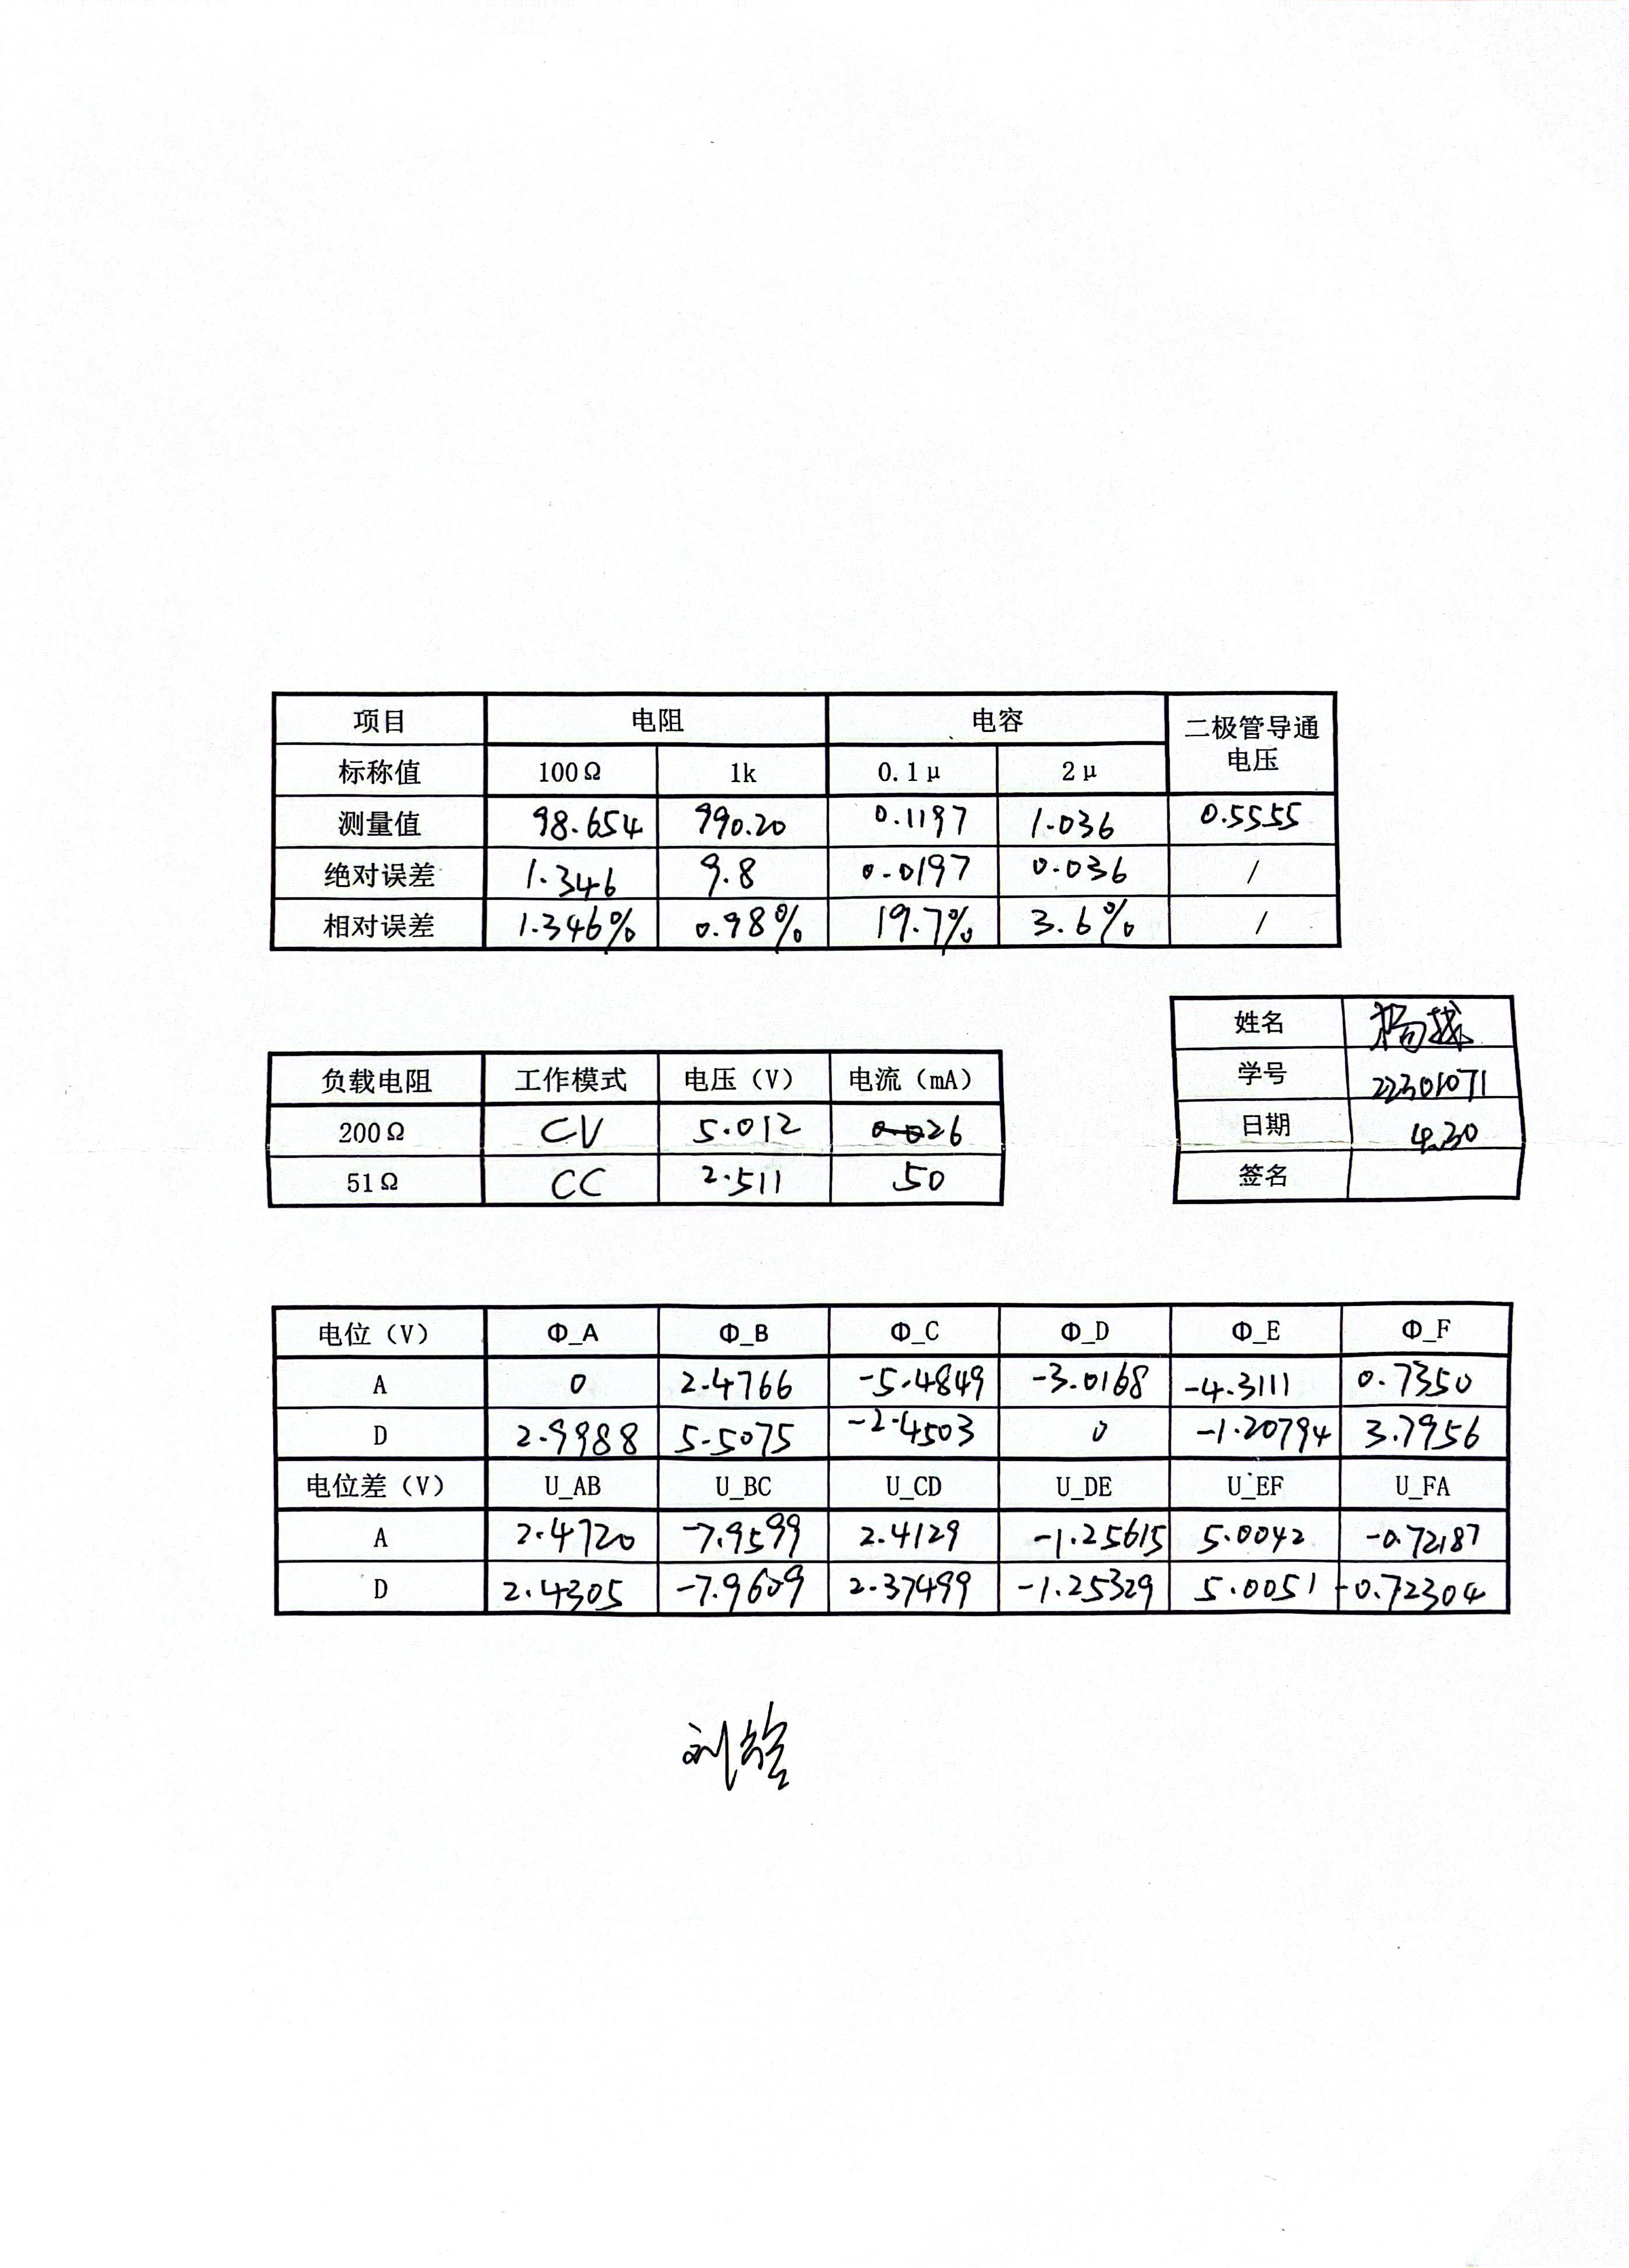
\includegraphics[width=\textwidth]{3}\\
\end{center}

\end{document}
